\documentclass[12pt]{article}

\usepackage[utf8]{inputenc}
\usepackage[T1]{fontenc}  
\usepackage{hyperref}    
\usepackage{url}   
\usepackage{graphicx}
\usepackage{tabularx}
\usepackage{mathptmx}
\usepackage[romanian]{babel}
\usepackage{indentfirst}
\usepackage{subfig}

\graphicspath{ {./graphics/} }

\hypersetup{
	colorlinks=true,
	linkcolor=blue,
	filecolor=magenta,      
	urlcolor=cyan,
}
\urlstyle{same}

\newcolumntype{C}[1]{>{\centering\arraybackslash}p{#1}}


\title{\textbf{Raport inițial - Automatic 2D-to-3D image conversion}}

\author{
 	ECHIPĂ: E6
	\\
	 Beldiman Vladislav Student1
	\\
	Grupa 1305A
}

\begin{document}

\noindent\begin{minipage}{0.1\textwidth}
	
\includegraphics[width=1.1cm]{logo_AC.png}
\end{minipage}
\hfill
\begin{minipage}{1\textwidth}\raggedright
	Universitatea Tehnică "Gheorghe Asachi" din Iași\\
	Facultatea de Automatică și Calculatoare\\
	Prelucrarea Imaginilor - Proiect
\end{minipage}

\vspace{5cm}
{\let\newpage\relax\maketitle}
\newpage

\section{Descrierea temei}

Obiectivul acestui proiect este de a crea o aplicație Windows cu interfață grafică care realizează conversia unei imagini din 2D în 3D cu interacțiune minimă în cadrul acestui proces din partea utilizatorului. Acest lucru va fi realizat considerând intensitatea fiecărui pixel drept valoarea înălțimii acestuia într-un câmp de înălțimi, iar pe baza acestor valori va fi construită o plasă poligonală cu fețe triunghiulare (Figura \ref{fig:fig1}).

Aplicația va fi scrisă în limbajul de programare C++ cu interfața grafică realizată cu ajutorul setului de instrumente Qt. Ea va permite vizualizarea imaginii încărcate și finale, cât și salvarea imaginii 3D în format STL.

Utilizatorul va avea la dispoziție câteva opțiuni precum adăugarea unui chenar la imaginea finală, inversarea acesteia (răsturnarea valorilor din câmp) sau selectarea altei erori maxime la triangulație.

Triangulația domeniului determinat de pixeli va fi realizată prin triangulația naivă (Figura \ref{fig:fig2}) care include toate punctele corespunzătoare pixelilor, sau prin aproximare prin înserare lacomă (Figura \ref{fig:fig3}) aplicând triangulația Delaunay sau triangulația dependentă de date cu unele optimizări [1]. Înserarea lacomă va folosi drept măsură de importanță pentru fiecare punct eroarea verticală dintre valoarea câmpului și aproximarea interpolată în acel punct.

\begin{figure}[h!]
	\caption{Exemplu de plasă poligonală rezultantă. [1]}
	\centering
	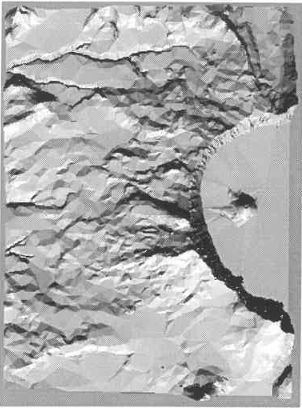
\includegraphics[width=0.4\linewidth]{ExempluPlasa.png}
	\label{fig:fig1}
\end{figure}

\begin{figure}[h!]
	\caption{Exemplu de triangulație naivă. [1]}
	\centering
	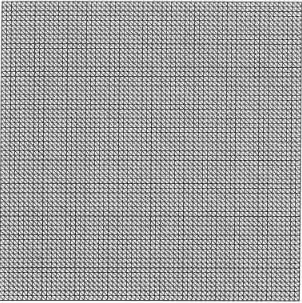
\includegraphics[width=0.6\linewidth]{ExempluTriangulatieNaiva.png}
	\label{fig:fig2}
\end{figure}

\begin{figure}[h!]
	\caption{Exemplu de triangulație care aproximează un câmp de înălțimi. [1]}
	\centering
	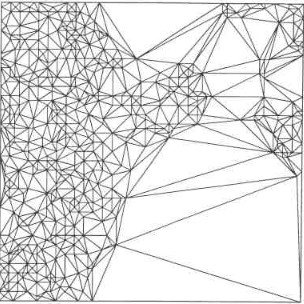
\includegraphics[width=0.6\linewidth]{ExempluTriangulatieCuAproximari.png}
	\label{fig:fig3}
\end{figure}

\clearpage
\section{Modalitatea de lucru propusă}%\textsuperscript{\tiny1}}

\begin{center}
	\begin{tabular}{|C{0.3cm}|C{10cm}|C{2cm}|C{2cm}|} 
		\hline
		\textbf{\#} & \textbf{Descriere sarcină} & \textbf{Stare} & \textbf{Membru} \\ 
		\hline
		1 & Documentare despre conversia imaginilor din 2D în 3D & în progres &  m1 \\ 
		\hline
		2 & Documentare despre Qt & în progres &  m1  \\ 
		\hline
		3 & Implementarea și testarea unei interfețe grafice minimaliste & în progres &  m1 \\ 
		\hline
		4 & Implementarea și testarea algoritmului naiv & - &  m1 \\ 
		\hline
		5 & Extinderea interfeței grafice cu opțiuni și testarea acestora & - &  m1 \\ 
		\hline
		6 & Implementarea și testarea algoritmului bazat pe triangulația Delaunay & - &  m1 \\
		\hline
		7 & Întocmirea raportului intermediar & - &  m1 \\
		\hline
		8 & Implementarea și testarea algoritmului bazat pe triangulația dependentă de date & - &  m1 \\
		\hline
		9 & Documentare despre formatul STL & - &  m1 \\
		\hline
		10 & Implementarea și testarea opțiunii de salvare în format STL a imaginii 3D & - &  m1 \\
		\hline
		11 & Rafinare și optimizări & - &  m1 \\ 
		\hline
		12 & Identificarea unui set potrivit de imagini (preferabil găsirea unei surse cu rezultate experimentale împreună cu probele folosite) & - & m1 \\
		\hline
		13 & Adăugarea posibilității de cronometrare a timpului de conversie & - &  m1 \\ 
		\hline
		14 & Realizarea experimentelor & - &  m1 \\ 
		\hline
		15 & Întocmirea raportului final & - &  m1 \\ 
		\hline
		16 & Pregătirea prezentării & - &  m1 \\ 
		\hline
	\end{tabular}
\end{center}

%{\tiny\textsuperscript{1}Unele sarcini, precum documentarea, nu vor fi realizate decât la finalul proiectului.}

\medskip

\textbf{Git repository:} \url{https://github.com/veeyslaw/hfbm}

\section*{Referințe}

\medskip

[1] \href{http://reports-archive.adm.cs.cmu.edu/anon/anon/home/ftp/1995/CMU-CS-95-181.pdf} {Garland M. and Heckbert P. S. (1995) Fast Polygonal Approximation of Terrains and Height Fields. (CMU-CS-95-181)}

\end{document}